\begin{figure}[t]
\begin{center}
	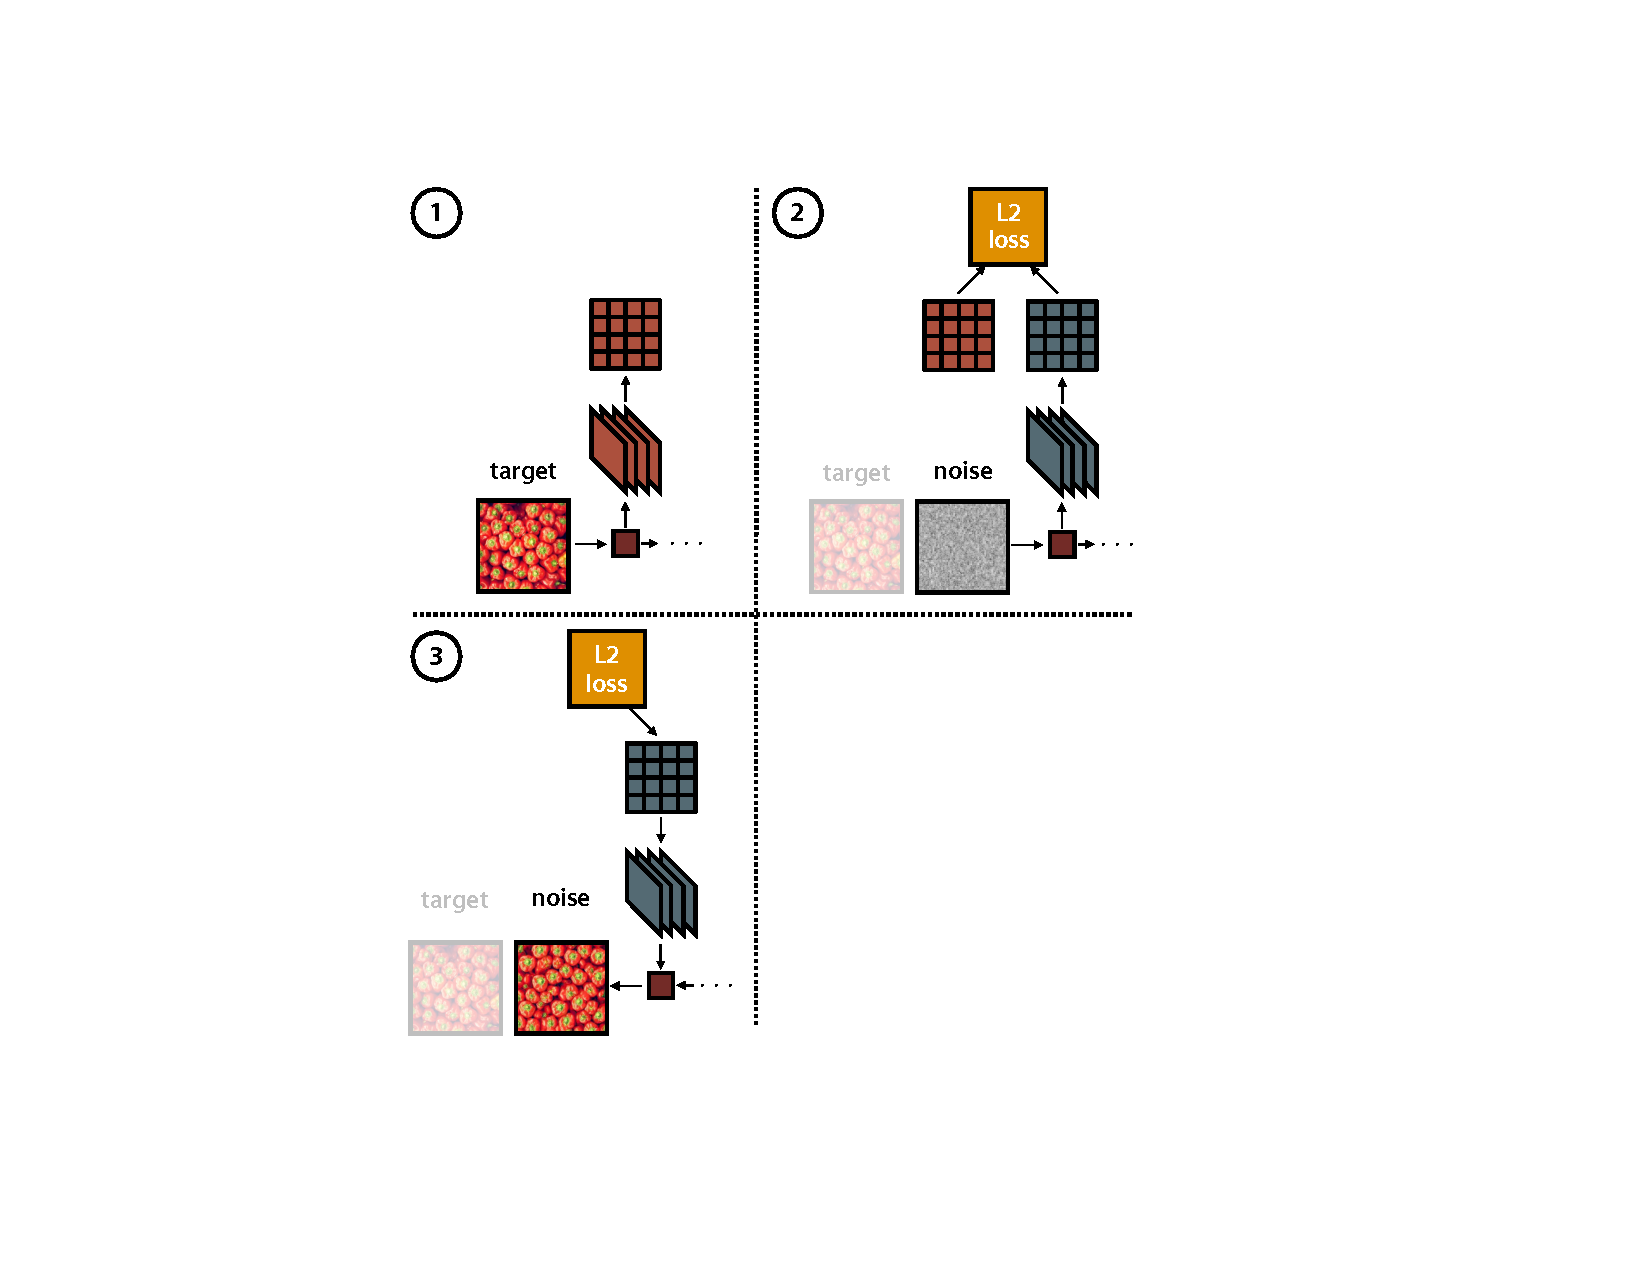
\epsfig{file=vgg_texture_synthesis.pdf, width = \textwidth}\\
	\caption[Static texture synthesis with a convolutional network]{Gatys \etal's \cite{gatys2015} approach to static texture synthesis with the VGG-19 \cite{simonyan2014very} convolutional network. Only the first layer of VGG-19 is shown. (1) An initial forward pass is
performed with the target texture. Its Gram matrices
across various layers are computed and stored. (2) The total L2 loss between the Gram matrices of the synthesized texture and the target is computed. (3) The loss is optimized with respect to the synthesized texture (with the weights of VGG-19 fixed), updating it to appear as perceptually similar to the target as possible.}
	\vspace{-0.65cm}
	\label{fig:vgg_texture_synthesis}
\end{center}
\end{figure}